The Gear Train design problem is a classic multi-objective optimization
problem, for it encompasses a number of the challenges that a practical
real world optimization task may present. It involves a number of variables
of different types and a large number of equality and inequality
constraints. A number of objectives can be considered for the
optimization. This problem was analyzed in \citep{agogino90} to explain the
design process from an optimization perspective, and in \citep{debgt} to
prove the applicability of NSGA-II in complex optimization tasks. We
analyze the pareto-optimal solutions of this design-optimization problem to
discover chunks of optimal designs using our proposed procedure.


\section{Problem description}
\label{problem}
The objective of multi-speed gearbox design is to obtain different
specified speeds in the output shaft with fixed input shaft angular
velocity. The two-dimensional layout of a 18-speed gearbox with 18 gears is
shown in figure \ref{geartrain}. Gears in shafts 1, 3 and 5 can be
translated to mesh with corresponding gears in shafts 2, 4 and 6 to obtain
desired output speed. The input shaft speed is kept fixed at 1400 rpm. With
a ratio of 1.14 between consecutive output speeds, the $i^{th}$ desired
output speed would be $1400/(1.14)^{i-1}$.  The lowest desired speed is
thus $1400/(1.14)^{17} = 150$ rpm.

\begin{figure}[ht]\begin{center}
 \fbox{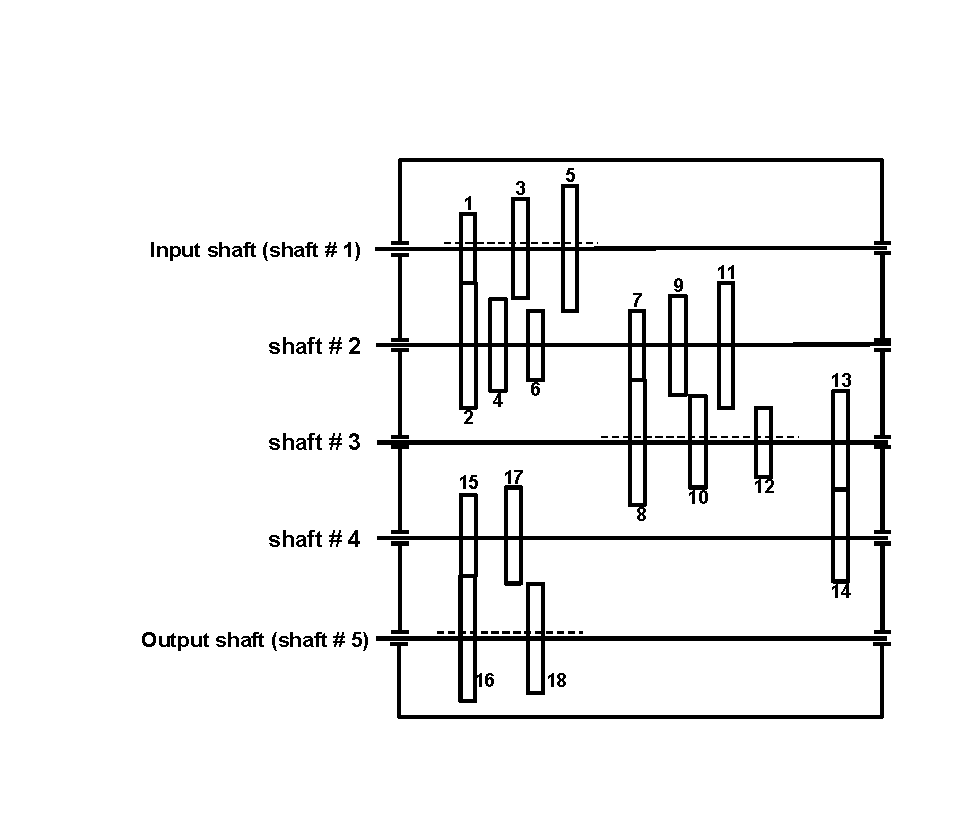
\includegraphics[width=80mm, height=65mm]{diagrams/geartrain.eps}}
 \caption{18-speed Gearbox layout. Gears in shafts 1, 3 and 5 can be
   translated to mesh with corresponding gears in shafts 2, 4 and 6
   respectively. With three different possible meshing of gears between
   shafts 1-2, 2-3 and two in shafts 2-4, 18 different output speeds are
   possible.}
 \label{geartrain}
\end{center}\end{figure}

A number of objectives can be considered for the design of the gear 
train design optimization, e.g.:
\begin{enumerate}[(i)]
\item minimization of the gear material used,
\item maximization of the power delivered, 
\item minimization of the error between desired and achieved output 
speeds.
\item minimization of the centre distance between input and output 
shaft,
\end{enumerate}
We will consider only the first three objectives in this study.

There are 29 variables over which an optimization problem can be defined:
\begin{enumerate}[(i)]
  \item thickness of gear-pairs, $t_i$ for $i = 1, 2, \dots 9$
  \item teeth module, the same for all the gear pairs,
  \item the power delivered $p$,
  \item the number of teeth in pinion of the $i^{th}$ gear-pair, 
  \item the number of teeth in wheel of the $i^{th}$ gear-pair, for $i = 1, 2, \dots 9$,
\end{enumerate}

To have varying number of teeth in the gears, the following 
constraints must be satisfied by all feasible gearbox designs:

\begin{enumerate}
  \item All mating gear-pairs on  two shafts should have the same 
   centre distances as the shaft distances.
  \item Since we have a two-dimensional gear-train layout, no gear 
   should interfere with any shaft.
  \item Maximum gear ratio in any gear pair should not exceed a limit
   $r^{max}$.
\end{enumerate}


% There are a large number of design parameters on which the optimization
% problem can be defined, depending on the aspects of the design we want to
% explore. 

The multi-objective formulation for the full problem is as follows:
\begin{singlespacing}
\begin{flushleft}


{\allowdisplaybreaks 
  \begin{align}
    \text{Maximize} \quad &f_1 =     \left. p,       \right.\\
    \text{Minimize} \quad &f_2 = \left. \frac{\pi m^2}{4} {\displaystyle\sum\limits_{i=1}^G {({n^2_{p_i}} + {n^2_{w_i}}) t_i }}\right.\\
    \text{Minimize} \quad &f_3 = \left. \max_{1 \le k \le 18}{|\Omega_k-{\Omega}_k^I|} \right. \\  
    \text{Subject to,}& \qquad  \left. \right.\nonumber \\
    &{\sigma}_{b_i} \leqslant  S_b \quad  &\left. \text{for} \quad i = 1, 2, \dots G, \right.\\
    &{\sigma}_{w_i} \leqslant S_w \quad   &\left. \text{for} \quad i = 1, 2, \dots G, \right.\\
    &t^{(L)} \leqslant t_i \leqslant t^{(U)}   &\left. \text{for} \quad i = 1, 2, \dots G, \right.\\
    &p^{(L)} \leqslant p \leqslant p^{(U)} \\
    \nonumber \\
    &n_1 + n_2 = n_3 + n_4 = n_5 + n_6,  \quad &\left. \text{(between shaft 1 and 2)} \right.\nonumber\\
    &n_7 + n_8 = n_9 + n_{10} = n_{11} + n_{12}, \quad &\left. \text{(between shaft 2 and 3)} \right.\nonumber\\
    &n_{15} + n_{16} = n_{17} + n_{18} \quad &\left. \text{(between shaft 4 and 5)} \right.\\
    \nonumber\\
    &n_2 \leqslant n_7 + n_8, \quad n_4 \leqslant n_7 + n_8, \nonumber\\
    &n_6 \leqslant n_7 + n_8, \quad n_7 \leqslant n_1 + n_2, \\
    \nonumber\\
    &n_9 \leqslant n_1 + n_2, \quad n_{11} \leqslant n_1 + n_2, \nonumber\\
    &n_8 \leqslant n_{13} + n_{14}, \quad n_{10} \leqslant n_{13} + n_{14},\\
    \nonumber\\
    &n_{12} \leqslant n_{13} + n_{14}, \quad n_{13} \leqslant n_7 + n_8, \nonumber\\
    &n_{14} \leqslant n_{15} + n_{16}, \quad n_{15} \leqslant n_{13} + n_{14},\\
    \nonumber\\
    &n_{17} \leqslant n_{13} + n_{14}\\
    \nonumber\\
    &\frac{n_{w_i}} {n_{p_i}}  \leqslant r^{max} \quad &\left. \text{(for i = 1, 2, \dots G)} \right.\nonumber\\
    &n_{w_i} \geqslant n^{(L)} &\left. \text{(for i = 1, 2, \dots G)} \right.\nonumber\\
    &n_{p_i} \geqslant n^{(L)} &\left. \text{(for i = 1, 2, \dots G)} \right.\nonumber\\
    &n_i \in \mathbb{Z} &\left. \text{(for i = 1, 2, \dots 2G)} \right. 
  \end{align}
}
Where, 

\end{flushleft}

\begin{itemize}
\item $m$ is the teeth module for all the gear pairs,
\item $n_{p_i}$ and $n_{w_i}$ are the number of teeth in the pinion 
and wheel in the $i^{th}$ gear-pair,
\item $t_i$ is the thickness of the gear-pair in cm., 
\item $\Omega_k$ is the actual $k^{th}$ output speed and $\Omega_k^I$ is the ideal $k^{th}$ output speed,
\item ${\sigma}_{b_i}$ is the bending stress developed in a gear-pair 
calculated as follows:

\begin{equation}
\sigma_{b_{i}} = \frac{97500 p { } k_c { } k_d { } (r_i + 1)} {a_{ i} { } {\omega}_{ i} { } t_{ i} { } m { } r_{ i} { } y_{ i} { } \text{cos} \beta} \\
\end{equation}

\item $S_b$ ($= 2,500\text{ kgf}/\text{cm}^2$) is the permissible bending stress,

\item ${\sigma}_{w_i}$ is the wearing stress developed in a gear-pair
calculated as follows:

\begin{equation}
\sigma_{w_{i}} = \frac{0.59 (r_i+1)}{r_i a_i} \sqrt{\frac{97500 p { } k_c { } k_d { } E (r_i + 1)}{ {\omega}_i t_i \text{sin} 2 \beta}}
\end{equation}
\item $S_w$ ($= 17,500\text{ kgf}/\text{cm}^2$) is the permissible wearing stress,

\item $k_c(=1.5)$ is the stress concentration factor,
\item $k_d(=1.1)$ is the dynamic load factor,
\item $r_i$ is the transmission ratio, defined as the ratio of number 
of teeth in the wheel $(n_{w_i})$ to the number of teeth in the 
pinion $(n_{p_i})$ for the $i^{th}$ gear-pair,
\item ${\omega}_i$ is the angular velocity of the wheel in rpm,
\item $a_i$ is the centre distance for the corresponding gear pair
given as 
\\
$a_i = \frac {m ( n_{w_i} + n_{p_i})} {2}$ , 
\item $y_i$ is the form load factor defined as 
$y_i = 0.52(1+ \frac{20}{n_{w_i}} )$ , 
\item ${\beta}(= 20 \text{ degrees})$ is the pressure angle,
\item $E $ ($= 2.1 \times 10^6\text{ kgf}/\text{cm}^2$) is the Young's modulus of the gear material. .
\end{itemize}

\end{singlespacing}

Here we will consider two instances of the problem:
\begin{enumerate}[(A)]
\item 11 variable problem in which thickness of all the gear-pairs and
  gear-module thickness are variable and only first two objectives are
  considered, and
\item the full problem.
\end{enumerate}

For the instance (A), the number of gear teeth layout is fixed to the
configuration given in table \ref{gearTeeth}. Constraints 3.8 onwards are
not applicable for this instance of the problem.

\begin{table}[!ht]
  \centering
  \begin{tabular}{|c|c|c|c|c|c|c|c|c|c|}
    \hline
    $i$ & 1 & 2 & 3 & 4 & 5 & 6 & 7 & 8 & 9  \\
    \hline
    \multicolumn{1}{|c|}{$n_{p_i}$} & 20 & 33 & 28 & 32 & 34 & 33 & 33 & 20 & 26\\
    \hline
    \multicolumn{1}{|c|}{$n_{w_i}$} & 56 & 43 & 48 & 37 & 35 & 36 & 34 & 54 & 48\\
    \hline
  \end{tabular}
  \caption{No. of teeth for each gear-pair in fixed layout gear-train design.}
  \label{gearTeeth}
\end{table}





\subsection{NSGA-II formulation and the pareto-front}
We use the same NSGA-II formulation as in \citep{debgt} to obtain the
pareto-optimal solutions. For the 11 variables case we fix the 
gear-box layout by fixing the number of teeth in each gear to the 
values shown in table \ref{gearTeeth}. 



In second case we utilize the equality constraints given in equations 3.4
to eliminate five gear teeth variables. We code the gear teeth variables in
such a way so as to avoid evaluating permutations of same combinations of
gears in each transmission stage. Also, we condense similar constraints
into one constraint wherever possible. The probabilities of recombination
and mutation operator are 0.9 and 0.3 respectively for both the
optimization cases. For the 11 variables optimization, we run NSGA-II for
600 generations with a population size of 3000, and for 10000 generations
with 3000 initial population for the 29 variable case. NSGA-II yields 927
points in the pareto-front for the first case. The pareto-front for the 29
variables optimization has 989 points. The pareto-fronts are shown in
figures \ref{gt11Clusters} and \ref{gtvClusters}.


\section{Fixed transmission ratio problem}

Figure \ref{gt11rv} shows the Isomap residual variances for the
pareto-front of the fixed lay-out gearbox pareto-front. The largest drop in
the Isomap residual variance from 3 to 4 dimensional Isomap embedding. This
suggests the pareto-front may have an intrinsic dimensionality of four, and
we can expect to have clusters of dimensions lower than 4.

The PCA explained variance is shown in \ref{gt11ev}, which clearly shows
that the pareto-front is one dimensional in the parameter space. Table
\ref{first2GTPCs} shows the weights of five variables which have the
highest absolute component in in the first two principal components. The
thicknesses of the gear pairs in the final transmission stage are the
variables with the highest weight in the first principal component. Next
are the thickness of the second and fifth gear-pairs. In the second
principal component, the gear module is the most important
variable. Weights of all the other variables are  negligible in this
principal component.


% \begin{figure}[ht]\begin{center}
%  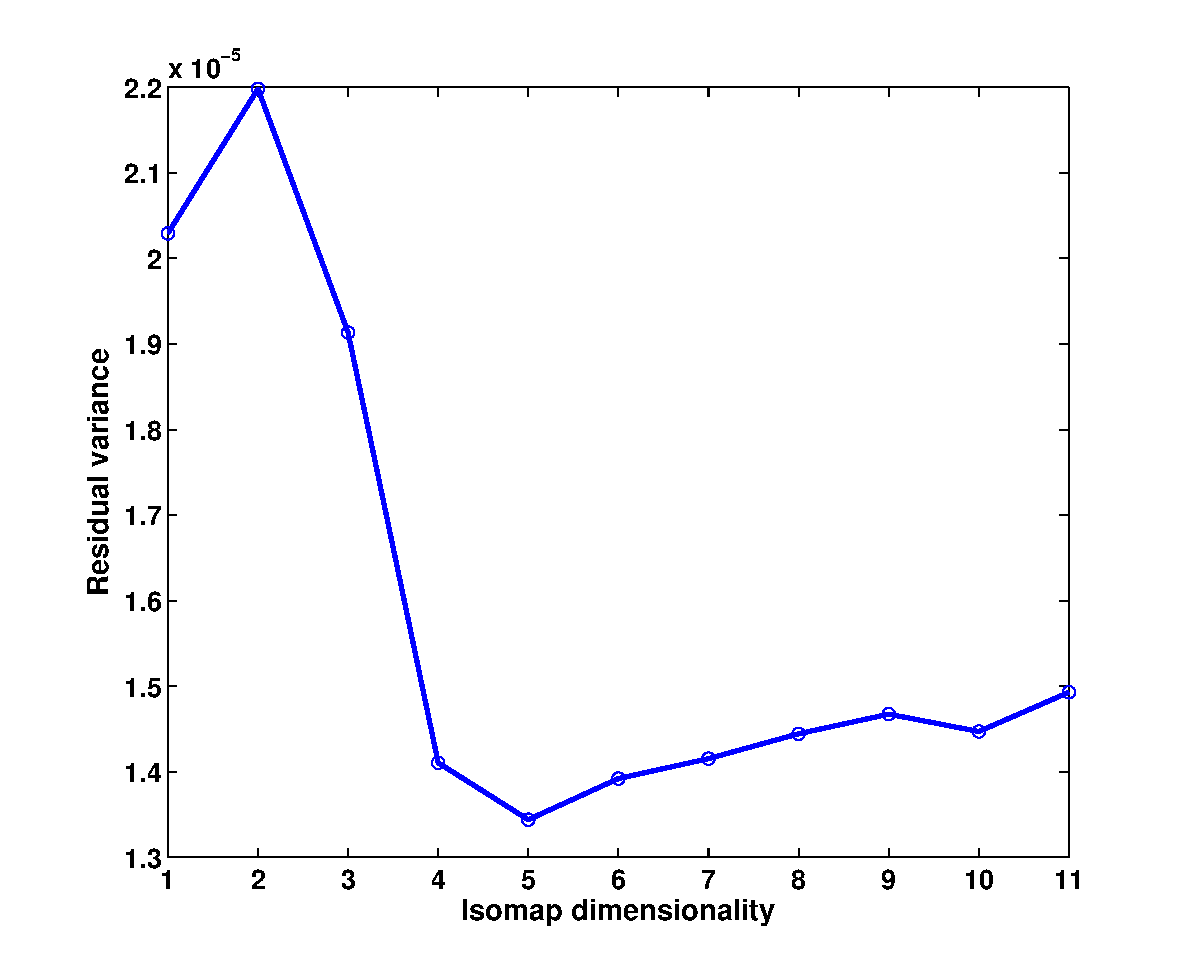
\includegraphics[width=100mm, height=80mm]{dia/gt11rv.eps}
%  \caption{Isomap residual variance for the fixed lay-out paret-front}
%  \label{gt11rv}
% \end{center}\end{figure}

\begin{figure}[ht]\begin{center}
 \subfloat[Isomap Residual Variance. ]{
 \label{gt11rv} 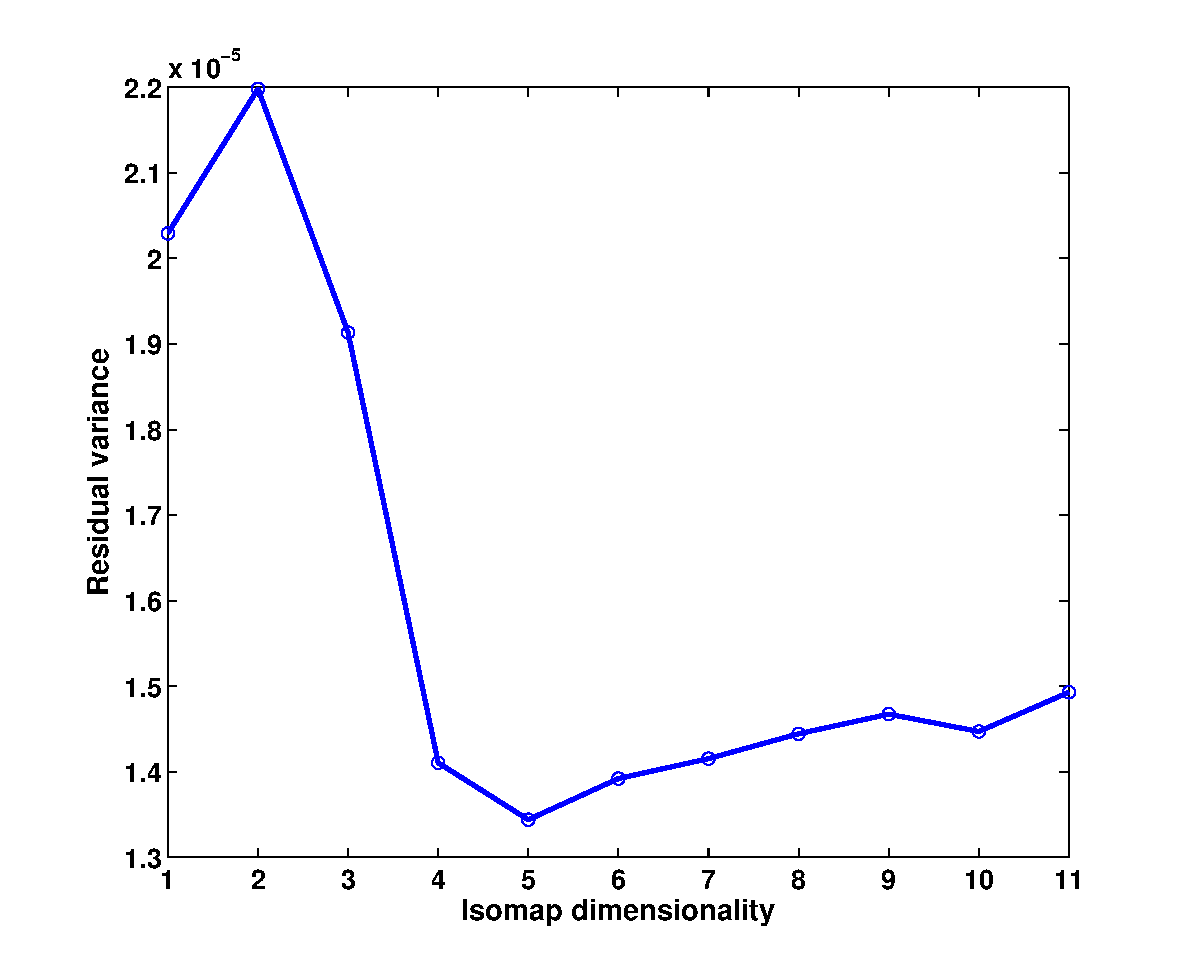
\includegraphics[width=62mm, height=52mm]{dia/gt11rv.eps}}
 \subfloat[PCA Explained variance.]{
 \label{gt11ev} 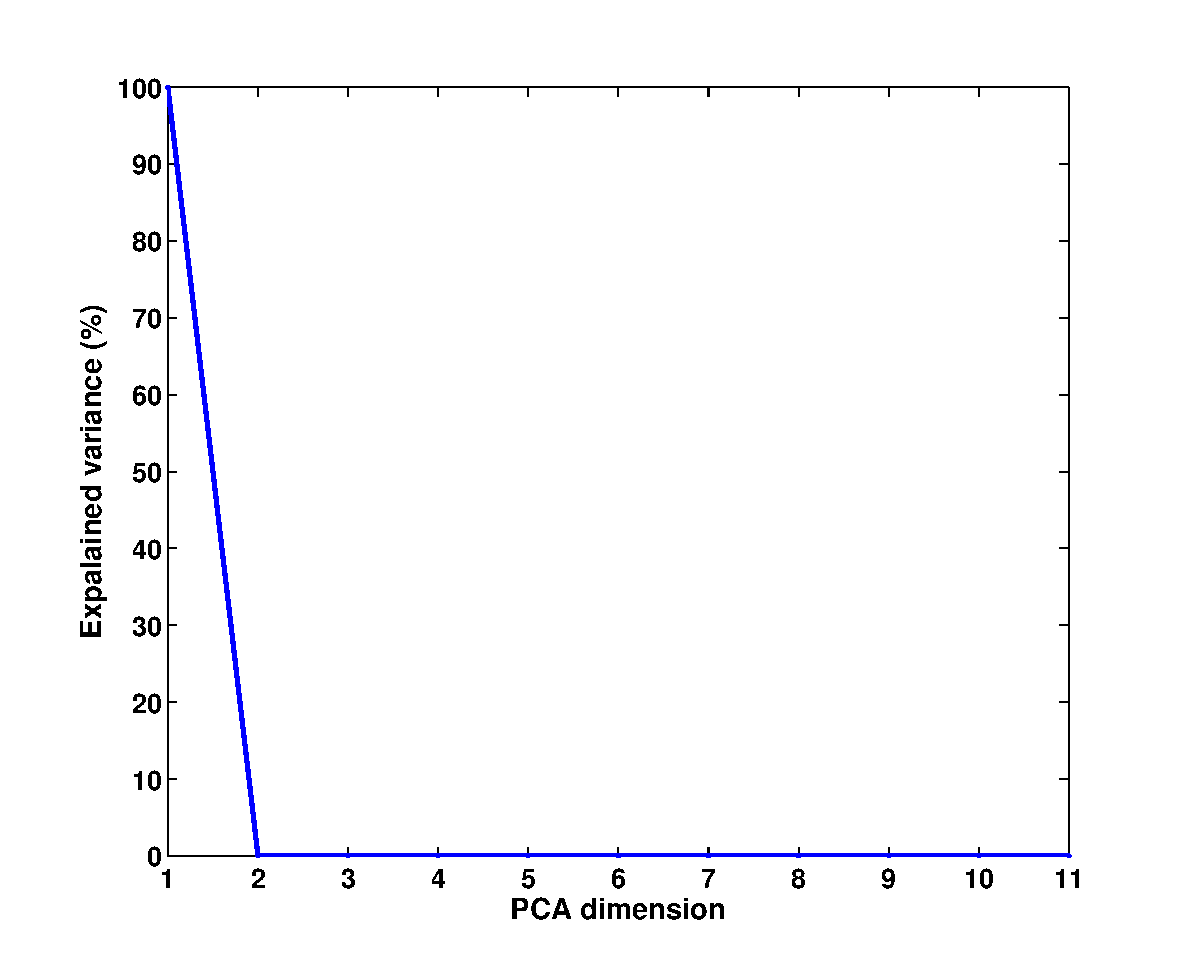
\includegraphics[width=62mm, height=52mm]{dia/gt11ev.eps}}
\caption{Isomap and PCA results for the fixed lay-out problem. The largest
  drop in residual variance is for the four dimensional Isomap
  embedding. The explained variance plot shows only one significant
  component.}
 \label{gt11rv}
\end{center}\end{figure}
 
\begin{table}[!ht]
  \centering
  \begin{tabular}{|c|c|c|c|c|c|}
    \hline
    \multirow{2}{*}{First PC}   & ($t_9$) &  ($t_8$) &  ($t_7$)  & ($t_6$) & ($p$)\\
    & -0.8444  & -0.4617  & 0.1837 & -0.1511 & 0.0733  \\
    \hline
    \multirow{2}{*}{Second PC}   & ($m$) &  ($t_5$) &  ($t_6$)  & ($t_9$) & ($t_8$)\\
    & 0.9997 & -0.0124 & 0.0097 & 0.0087 &  0.0087 \\
    \hline
  \end{tabular}
  \caption{First two principal components of the fixed layout gearbox pareto-front. $t_9$ and $t_8$ are the variables with the highest weights in the first component.}
  \label{first2GTPCs}
\end{table}

\subsection{Clustering the pareto-front}
Although it is possible to cluster the pareto-front into smaller clusters
by varying the $k$ parameter in our algorithm, we show and analyze
significantly sized and smaller number of clusters for the sake of
simplicity. Figure \ref{gt11Clusters} shows the 11 clusters obtained by
setting $k = 6.0$.

\begin{figure}[ht]\begin{center}
 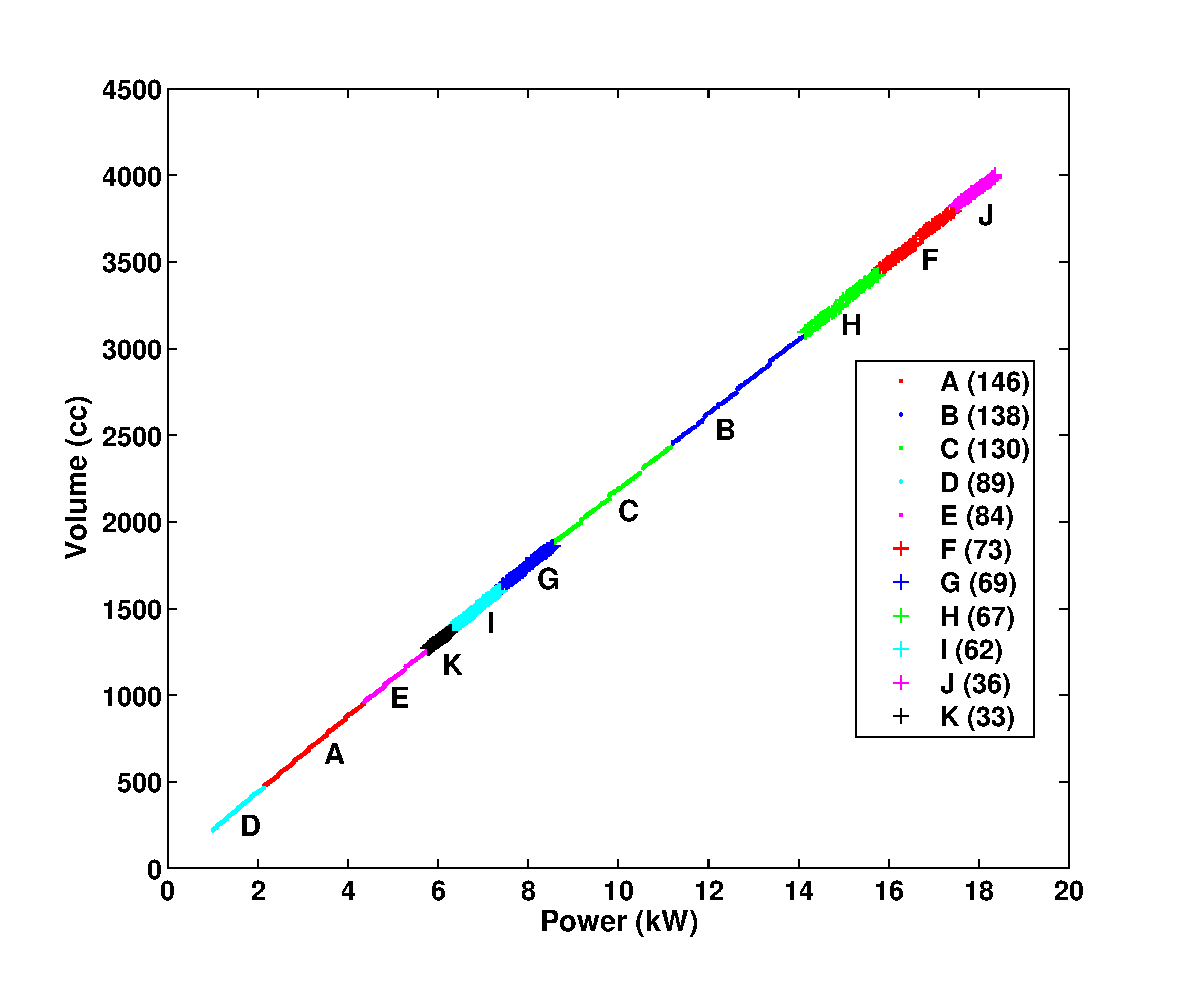
\includegraphics[width=100mm, height=80mm]{dia/gt11cpareto1.eps}
 \caption{Fixed layout gearbox design pareto-front and clusters in the
   objective space. There are 927 solutions in the pareto-front. The
   clusters in the extremes of the pareto-front are small.}
 \label{gt11Clusters}
\end{center}\end{figure}

\subsubsection{Isomap and PCA analysis}

The Isomap residual variance for most of the clusters is negligible except
for the cluster \textbf{D} for the residual variance is plotted in figure
\ref{gt11clustersrv}. The largest drop in residual variance is observed for
the second Isomap dimension after which it is constant, suggesting a
manifold dimensionality of one. All the clusters thus have a manifold
dimensionality of one, conforming to the {\em chunk dimensionality
  conjecture}. PCA analysis shows that clusters \textbf{B}, \textbf{C},
\textbf{F}, \textbf{J} and \textbf{K} are clearly one dimensional with the
first principal component of these clusters having explained variance of
more than 99\%. For the cluster \textbf{D}, the first principal component
has an explained variance of 80\% while the second principal component has
20\%. Figure \ref{gt11ev} shows the explained variance plot of cluster
\textbf{D} along with other clusters whose first components have explained
variance less than 99\%.

 



\begin{figure}[ht]\begin{center}
    \subfloat[Isomap Residual Variance for the cluster \textbf{D}.]{
      \label{gt11clustersrv} 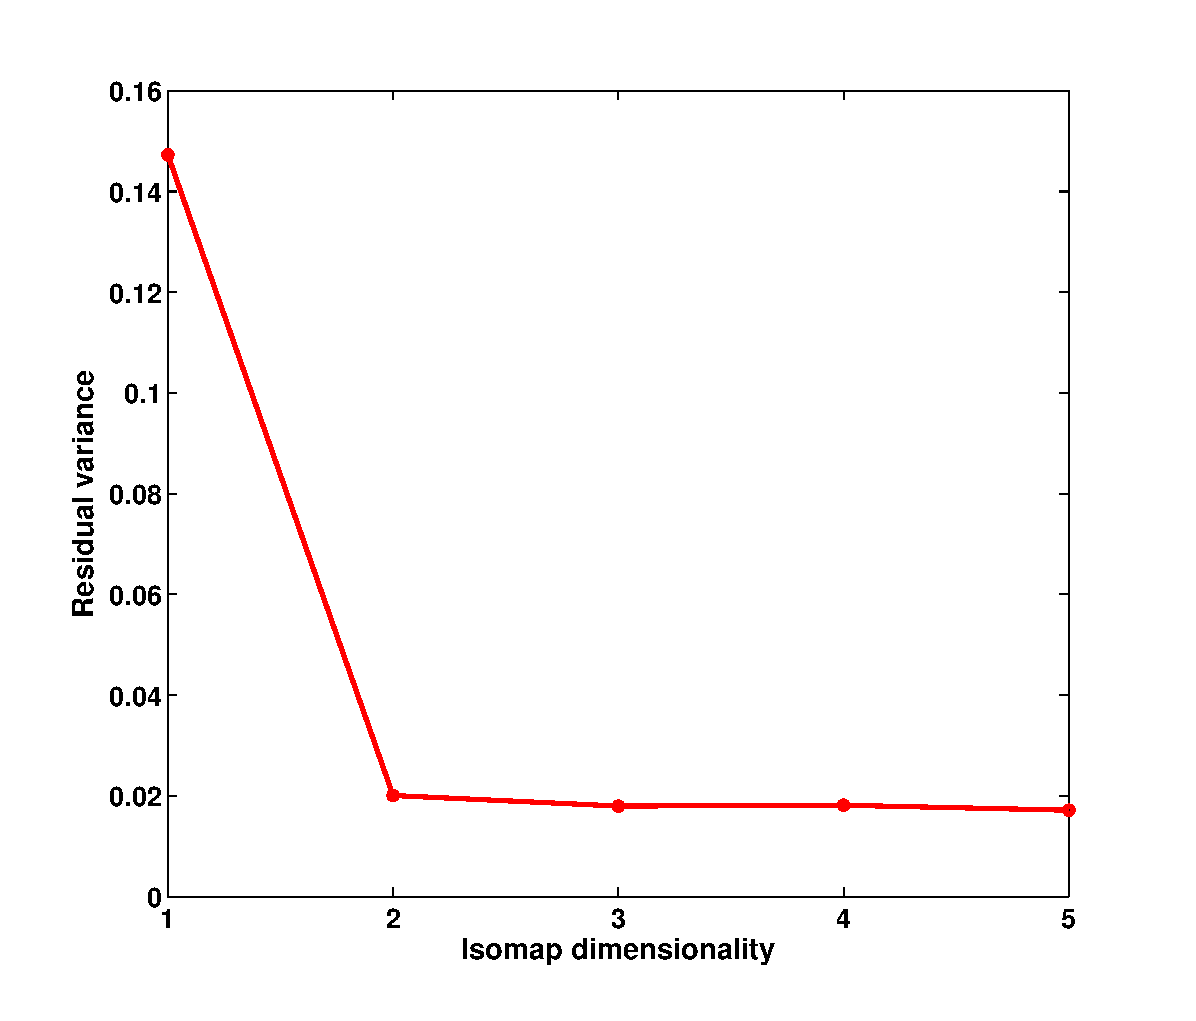
\includegraphics[width=62mm, height=52mm]{dia/gt11cluster4rv.eps}}
    \subfloat[PCA Explained variance for some of the clusters.]{
      \label{gt11clustersev} 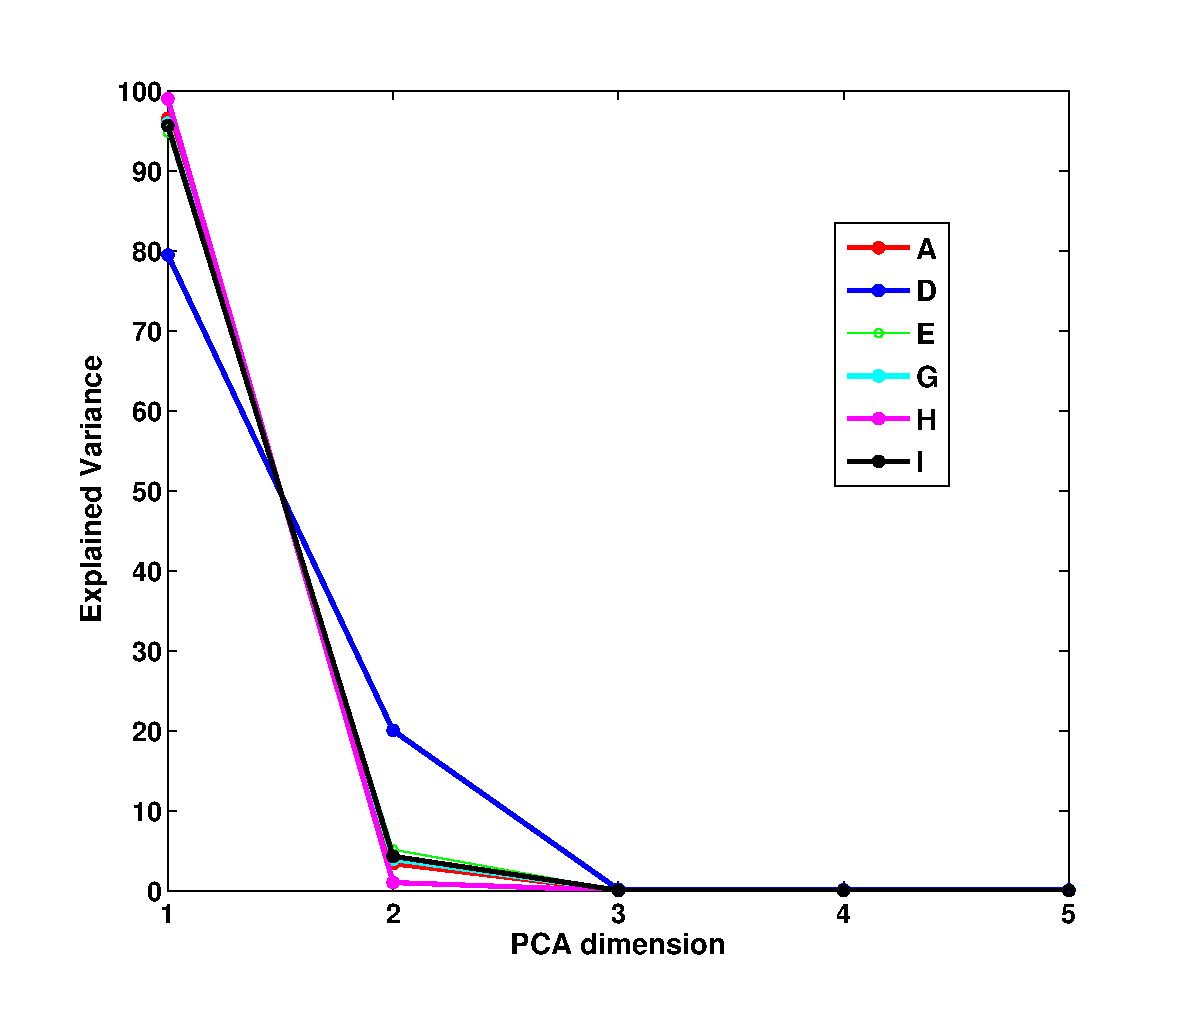
\includegraphics[width=62mm, height=52mm]{dia/gt11clustersEV.eps}}
    \caption{Isomap and PCA results for the clusters of fixed lay-out
      problem. \textbf{D} has the largest residual variance, all other
      clusters have negligible residual variances. The plot indicates a one
      dimensional manifold. Only cluster \textbf{D} has two significant
      principal component, all others have only one significant principal
      component.}
    \label{gt11clustersVar}
  \end{center}
\end{figure}


{\tiny

  {\small
    \begin{table}[!ht]
      \centering
      \begin{tabular}{|c|c|c|c|c|c|c|c|c|c|c|c|}
        \hline
        \multirow{2}{*}{\textbf{A}}   & $p$ & \cellcolor[gray]{0.45} $t_8$ & \cellcolor[gray]{0.50} $t_9$  & $m$ & \cellcolor[gray]{0.65} $t_7$ & \cellcolor[gray]{0.60} $t_4$ & \cellcolor[gray]{0.70} $t_5$ & \cellcolor[gray]{0.75} $t_6$ & \cellcolor[gray]{0.40} $t_1$ & \cellcolor[gray]{0.80} $t_3$ & \cellcolor[gray]{0.55} $t_2$ \\
        & 0.99  & 0.04  & 0.02 & 0.02 & 0.01 & 0.01 & 0.01 & 0.01 & 0.00 & 0.00 & 0.00 \\
        \hline
        \multirow{2}{*}{\textbf{B}}   & $p$ & \cellcolor[gray]{0.45} $t_8$ &  $m$  & \cellcolor[gray]{0.50}$t_9$ & \cellcolor[gray]{0.65} $t_7$ & \cellcolor[gray]{0.60} $t_4$ & \cellcolor[gray]{0.70} $t_5$ & \cellcolor[gray]{0.75} $t_6$ & \cellcolor[gray]{0.40} $t_1$ & \cellcolor[gray]{0.80} $t_3$ & \cellcolor[gray]{0.55} $t_2$ \\
        & 0.99 & 0.01 & 0.01 & 0.01 &  0.00 & 0.00 & 0.00 & 0.00 & 0.00 & 0.00 & 0.00 \\
        \hline
        \multirow{2}{*}{\textbf{C}} & $p$ & \cellcolor[gray]{0.45} $t_8$ & \cellcolor[gray]{0.50} $t_9$ &  $m$ & \cellcolor[gray]{0.65} $t_7$ & \cellcolor[gray]{0.60} $t_4$ & \cellcolor[gray]{0.70} $t_5$ & \cellcolor[gray]{0.75} $t_6$ & \cellcolor[gray]{0.40} $t_1 $ & -- & -- \\
        & 0.99 & 0.02 & 0.01 & 0.01 & 0.01 & 0.01 & 0.01 & 0.01 & 0.01 & 0 & 0 \\
        \hline
        \multirow{4}{*}{\textbf{D}} & $p$ & \cellcolor[gray]{0.45} $t_8$ & \cellcolor[gray]{0.50} $t_9$ &  \cellcolor[gray]{0.65} $t_7$ & $m$ & \cellcolor[gray]{0.60} $t_4$ & \cellcolor[gray]{0.70} $t_5$ & \cellcolor[gray]{0.75} $t_6$ &\cellcolor[gray]{0.40} $t_1$ &\cellcolor[gray]{0.80} $t_3$ & \cellcolor[gray]{0.55} $t_2$ \\
        & 0.99 & 0.07 & 0.06 & 0.03 & 0.03 & 0.03 & 0.03 & 0.02 & 0.02 & 0.00 & 0.00 \\ 
        \cline{2-12}
        & \cellcolor[gray]{0.45} $t_8$ & \cellcolor[gray]{0.50} $t_9$ & \cellcolor[gray]{0.65} $t_7$ &  \cellcolor[gray]{0.60} $t_4$ & \cellcolor[gray]{0.70} $t_5$ & \cellcolor[gray]{0.75} $t_6$ & \cellcolor[gray]{0.40} $t_1$ & $p$ & $m$ & \cellcolor[gray]{0.80} $t_3$ & \cellcolor[gray]{0.55} $t_2$ \\
        & -0.64 & -0.46 & -0.32 & -0.29 & -0.26 & -0.24 & 0.17 & 0.12 & 0.02 & 0.00 & 0.00 \\
        \hline
        \multirow{2}{*}{\textbf{E}} & $p$ & \cellcolor[gray]{0.45} $t_8$ & \cellcolor[gray]{0.50} $t_9$ &  \cellcolor[gray]{0.65} $t_7$ & \cellcolor[gray]{0.70} $t_5$ & \cellcolor[gray]{0.60} $t_4$ & \cellcolor[gray]{0.75} $t_6$ & $m$ & \cellcolor[gray]{0.40} $t_1$ & \cellcolor[gray]{0.80} $t_3$ & \cellcolor[gray]{0.55} $t_2$ \\
        & 0.99 & 0.07 & 0.05 & 0.03 & 0.02 & 0.02 & 0.02 & 0.01 & 0.01 & 0.00 & 0.00 \\ 
        \hline
        \multirow{2}{*}{\textbf{F}} & $p$ & \cellcolor[gray]{0.45} $t_8$ & \cellcolor[gray]{0.50} $t_9$ &  \cellcolor[gray]{0.65} $t_7$ & \cellcolor[gray]{0.60} $t_4$ & \cellcolor[gray]{0.75} $t_6$ & \cellcolor[gray]{0.70} $t_5$ & \cellcolor[gray]{0.40} $t_1$ & $m$ & \cellcolor[gray]{0.55} $t_2$ & \cellcolor[gray]{0.80} $t_3$ \\
        & 0.99 & 0.03 & 0.02 & 0.01 & 0.01 & 0.01 & 0.01 & 0.01 & 0.0 & 0.0 & 0.0 \\ 
        \hline
        \multirow{2}{*}{\textbf{G}} & $p$ & \cellcolor[gray]{0.45} $t_8$ & \cellcolor[gray]{0.50} $t_9$ & \cellcolor[gray]{0.65} $t_7$ & \cellcolor[gray]{0.75} $t_6$ & \cellcolor[gray]{0.60} $t_4$ & \cellcolor[gray]{0.70} $t_5$ & \cellcolor[gray]{0.40} $t_1$ & $m$ & \cellcolor[gray]{0.80} $t_3$ & \cellcolor[gray]{0.55} $t_2$ \\
        & 0.99 & 0.07 & 0.05 & 0.04 & 0.03 & 0.03 & 0.03 & 0.02 & 0.01 & 0.0 & 0.0 \\ 
        \hline
        \multirow{2}{*}{\textbf{H}} & $p$ & \cellcolor[gray]{0.45} $t_8$ & \cellcolor[gray]{0.50} $t_9$ & \cellcolor[gray]{0.60} $t_4$ &\cellcolor[gray]{0.65} $t_7$ &\cellcolor[gray]{0.70} $t_5$ &\cellcolor[gray]{0.75} $t_6$ &\cellcolor[gray]{0.40} $t_1$ & $m$ & -- & -- \\
        & 0.99 & 0.04 & 0.03 & 0.02 & 0.01 & 0.01 & 0.01 & 0.01 & 0.00 & 0 & 0 \\ 
        \hline
        \multirow{2}{*}{\textbf{I}} & $p$ &\cellcolor[gray]{0.45} $t_8$ & \cellcolor[gray]{0.50} $t_9$ & \cellcolor[gray]{0.65} $t_7$ &\cellcolor[gray]{0.60} $t_4$ &\cellcolor[gray]{0.70} $t_5$ &\cellcolor[gray]{0.75} $t_6$ &\cellcolor[gray]{0.40} $t_1$ & $m$ & -- & -- \\
        & 0.98 & 0.10 & 0.07 & 0.05 & 0.04 & 0.04 & 0.04 & 0.03 & 0.01 & 0 & 0 \\ 
        \hline
        \multirow{2}{*}{\textbf{J}} & $p$ &\cellcolor[gray]{0.45} $t_8$ &\cellcolor[gray]{0.50} $t_9$ & \cellcolor[gray]{0.65} $t_7$ & \cellcolor[gray]{0.60} $t_4$ &\cellcolor[gray]{0.75} $t_6$ &\cellcolor[gray]{0.70} $t_5$ &\cellcolor[gray]{0.40} $t_1$ &\cellcolor[gray]{0.80} $t_3$ &\cellcolor[gray]{0.55} $t_2$ & $m$ \\
        & 0.97 & 0.13 & 0.10 & 0.06 & 0.06 & 0.05 & 0.05 & 0.03 & 0.0 & 0.0 & 0 \\ 
        \hline
        \multirow{2}{*}{\textbf{K}} & $p$ &\cellcolor[gray]{0.45} $t_8$ & \cellcolor[gray]{0.50} $t_9$ & \cellcolor[gray]{0.65} $t_7$ &\cellcolor[gray]{0.60} $t_4$ &\cellcolor[gray]{0.70} $t_5$ &\cellcolor[gray]{0.75} $t_6$ &\cellcolor[gray]{0.40} $t_1$ &\cellcolor[gray]{0.80} $t_3$ &\cellcolor[gray]{0.55} $t_2$ & $m$ \\
        & 0.85 & 0.33 & 0.25 & 0.17 & 0.14 & 0.13 & 0.13 & 0.09 & -0.00 & -0.00 & 0 \\ 
        \hline
      \end{tabular}
      \caption{Principal component weights of each cluster in sorted order of absolute weights. Background shading indicates the input to output speeds for the gear pair. Darker cells indicate higher ratio. The gear pairs in the last transmission stage have the highest weights and those in the first transmission stage have the lowest weights for all the clusters.}
      \label{gt11pcTopWeights}
    \end{table}
  }
}
% & $t_$ & $t_$ & $t_$ & $t_$ & $t_$ & $t_$ 
% & 0.0 & 0.0 & 0.0 & 0.0 & 0.0 & 0.0 

Table \ref{gt11pcTopWeights} shows the top weights of the principal
components of the clusters. Only the first principal components for most of
the clusters are shown, as most of them have negligible explained variances
for subsequent principal components. Power is the predominant variable in
the principal components of all the clusters, followed by thickness of the
gear-pairs in the final transmission stage.  In larger clusters, module
occupies higher positions compared to smaller clusters.


\subsection{Discussion}
Apart from being a variable, power ($p$) is also one of the objectives of
the multi-objective optimization problem, taking a different value for each
pareto-optimal solution. This explains its highest weight in the principal
components of all the clusters. Next we have the thicknesses of gear-pairs
($t_i$) with module thickness ($m$) occupying various positions depending
on the size of the clusters. The positions of the thickness variables can
be explained on the basis of input to output speed ratio for each
gear-pair.  These ratios are shown in table \ref{iosRatio} in increasing
order. The gear-pairs having smaller input to output speed ratio should
have higher thickness as the pinion of these gear-pairs has to withstand
higher stresses.  The speed of the gear-pairs also inversely affects the
stress, the higher the speed the lower will be the stress for the same
power transmitted.



\begin{table}[!ht]
  \centering
  \begin{tabular}{|c|c|c|c|c|c|c|c|c|c|}
    \hline
    Gear pair No. & \cellcolor[gray]{0.40} 1 & \cellcolor[gray]{0.45} 8 & \cellcolor[gray]{0.50} 9 & \cellcolor[gray]{0.55} 2 & \cellcolor[gray]{0.60} 4 & \cellcolor[gray]{0.65} 7 & \cellcolor[gray]{0.70} 5 &\cellcolor[gray]{0.75} 6 & \cellcolor[gray]{0.80} 3\\
    \hline
    I/O Speed ratio & \cellcolor[gray]{0.40} 0.35 & \cellcolor[gray]{0.45} 0.46 & \cellcolor[gray]{0.50} 0.54 & \cellcolor[gray]{0.55} 0.76 & \cellcolor[gray]{0.60} 0.86 & \cellcolor[gray]{0.65} 0.97 & \cellcolor[gray]{0.70}0.97 & \cellcolor[gray]{0.75} 1.09 & \cellcolor[gray]{0.80} 1.71\\
    \hline
  \end{tabular}
  \caption{Gear pairs with lowest input to output speed ratios.}
  \label{iosRatio}
\end{table}


The positions of thickness variables in the principal components in table
\ref{gt11pcTopWeights} have been colour coded similar to table
\ref{iosRatio}. It can be observed that the thickness variables occur in
the order of the transmission stage they are in. $t_8$ and $t_9$ are the
thicknesses of the gears in the final transmission stage, $t_7$ in the
penultimate stage followed by $t_4$, $t_5$, $t_6$ and $t_1$, $t_2$, $t_3$
in the second and first stages.  The speeds would generally be the lowest
in the final transmission stage, consequently, the thicknesses in these
gear-pairs would have to be increased commensurate with the increasing
power. As opposed to this, the shafts in the first transmission stage will
have the highest speeds and the stresses will be the lowest, hence the
thickness of these gears generally stick to the lowest possible value of
0.5. Only for high power gear boxes do they show any variation, e.g.  in
clusters \textbf{J} and \textbf{F}, in which $t_1$ has higher absolute
weights than module ($m$). It can also be noticed that gear-pairs in the
same shaft are arranged in the order of increasing input to output ratio in
the principal components. Although $G_1$ has the lowest input to output
speed ratio, the position of $t_1$ in the principal components is after the
gear-pairs in other transmission stages. This suggests that the speed of
the gear pair is an important factor in stress and thickness of the
gear-pair.


\begin{figure}[ht]\begin{center}
 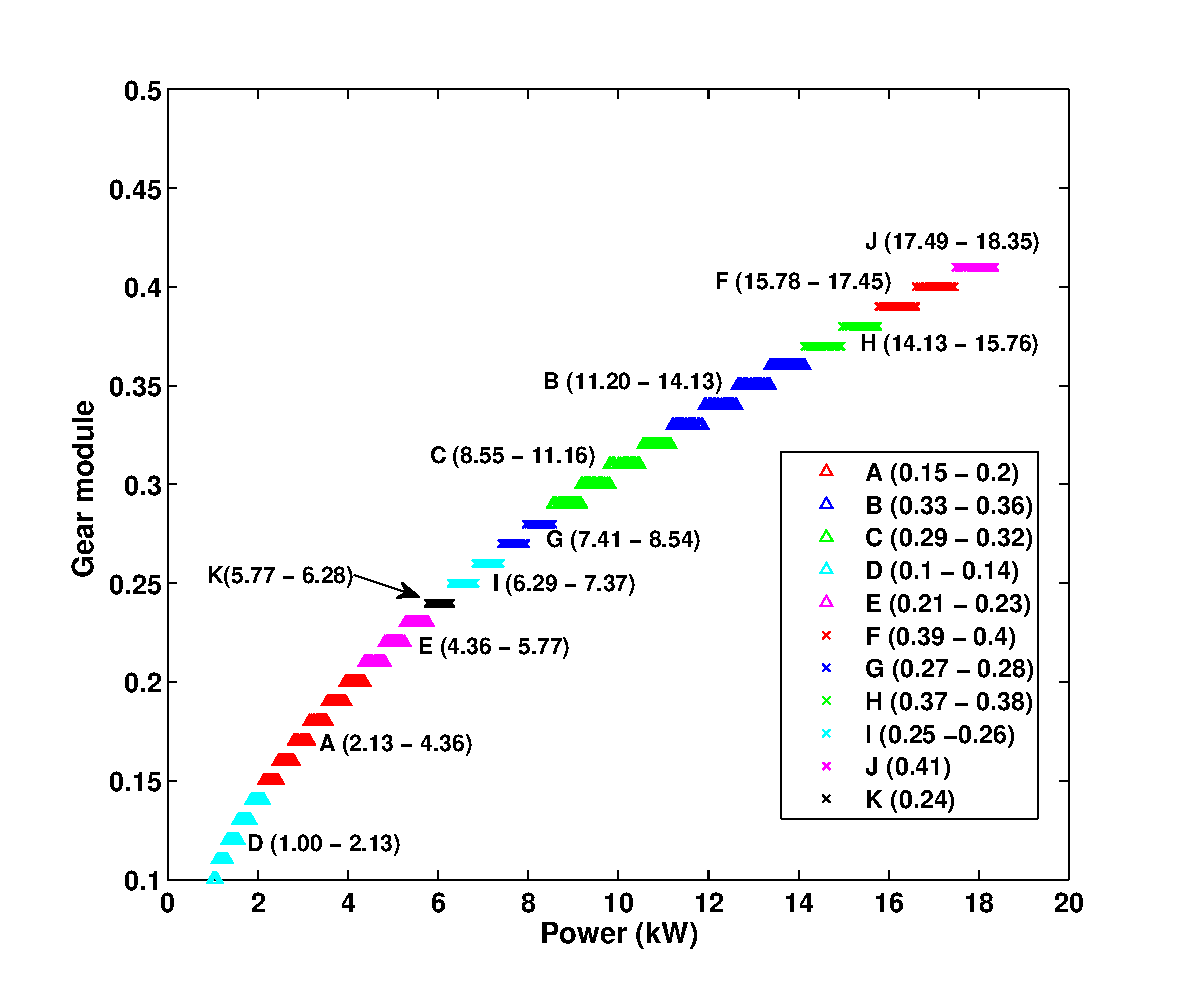
\includegraphics[width=100mm, height=80mm]{dia/gt11pVsm.eps}
 \caption{Power Vs. module characteristics of the pareto-front. Clusters occupy contiguous steps in the staircase structure.}
 \label{gt11pVsm}
\end{center}\end{figure}

Module weight in the principal components depends upon the size of the
cluster. For clusters \textbf{A}, \textbf{B}, \textbf{C} and \textbf{D},
$m$ occurs at positions up to fifth.  Figure \ref{gt11pVsm} shows the power
Vs. module plot for the clusters.  The staircase structure of this plot
shows that for a higher power gearbox a larger module is required. This
plot also explains the higher weights of $m$ variable in the clusters
mentioned earlier.  The cluster \textbf{A} is composed of designs with
five different module widths, cluster \textbf{B} and \textbf{C} with four,
and cluster \textbf{D} again with five different module widths. For these
clusters, module has a good range of variation hence the higher weights in
the principal components. On the other hand, clusters \textbf{J} and
\textbf{K} have designs with the same module width, their principal
components indicate this by having zero weights for $m$.




\section{29 Variable problem}

The pareto-front and the clusters obtained for the 29 variable problem
are shown in the figure \ref{gtvClusters}. As with the fixed layout problem,
we keep the size and number of clusters low by choosing a higher $k$ parameter 
value in our algorithm.


\begin{figure}[ht]\begin{center}
 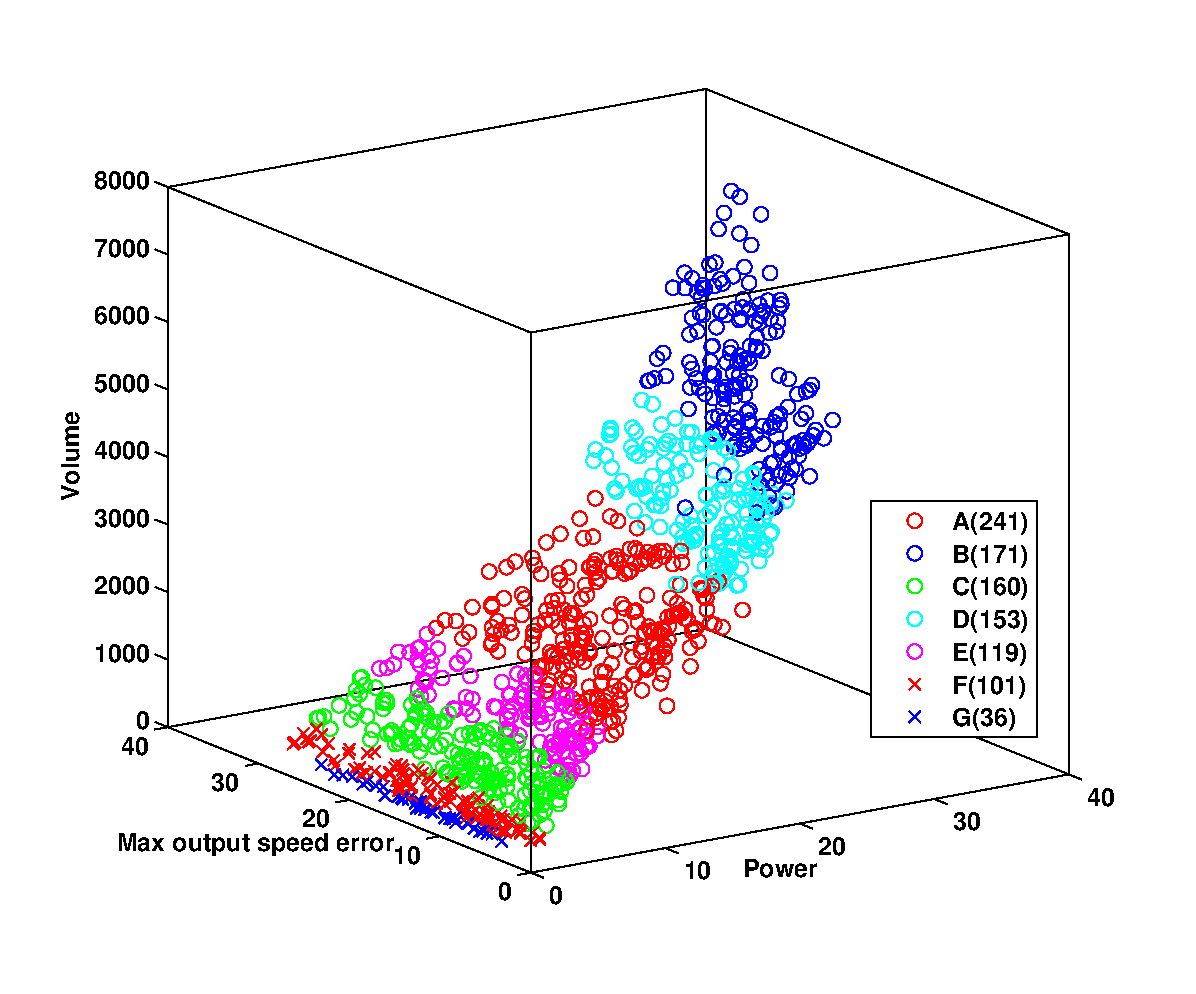
\includegraphics[width=100mm, height=80mm]{dia/gtvopareto2.eps}
 \caption{The pareto-front and the clusters for the 29-variable problem. The pareto-front manifold is clearly a two dimensional manifold in the objective space. }
 \label{gtvClusters}
\end{center}\end{figure}

Figure \ref{gtvRvEv} shows the Isomap residual variance and PCA explained
variances for the pareto-front. The residual variance plot gives no certain
indications about the dimensionality of the pareto-front. The largest drop
in residual variance occurs for second Isomap dimension and keeps dropping
up-to the fifth dimension after which it flattens out. The explained
variance also gives a similar picture; the explained variances for the
first, second, third and fourth principal components are 63.6\%, 11.6\%,
7.6\% and 7.1\% respectively. 


\begin{figure}[ht]\begin{center}
    \subfloat[Isomap Residual Variance.]{
      \label{gt11rv} 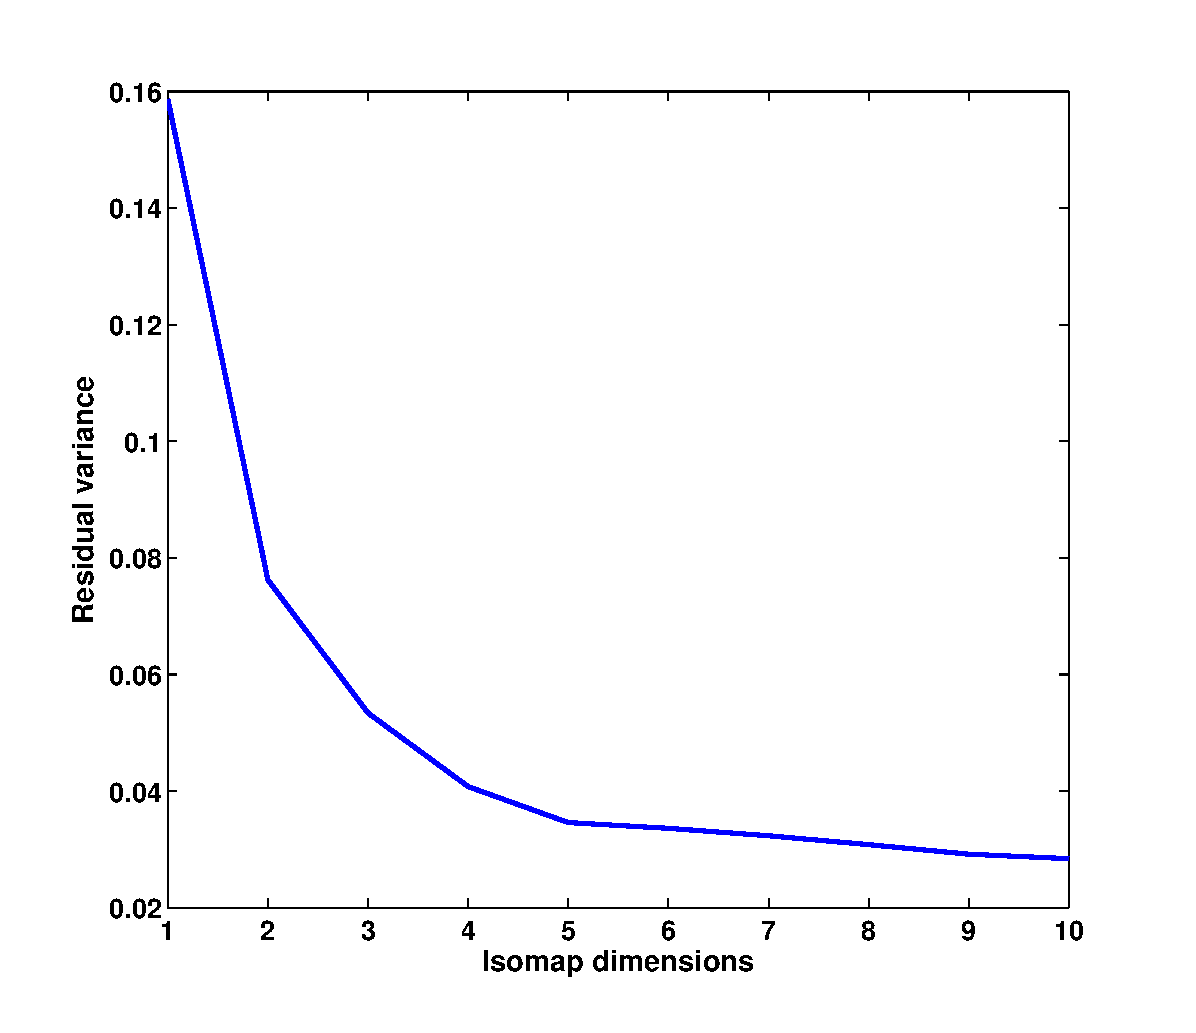
\includegraphics[width=62mm, height=52mm]{dia/gtvorv1.eps}}
    \subfloat[PCA explained variance.]{
      \label{gt11ev} 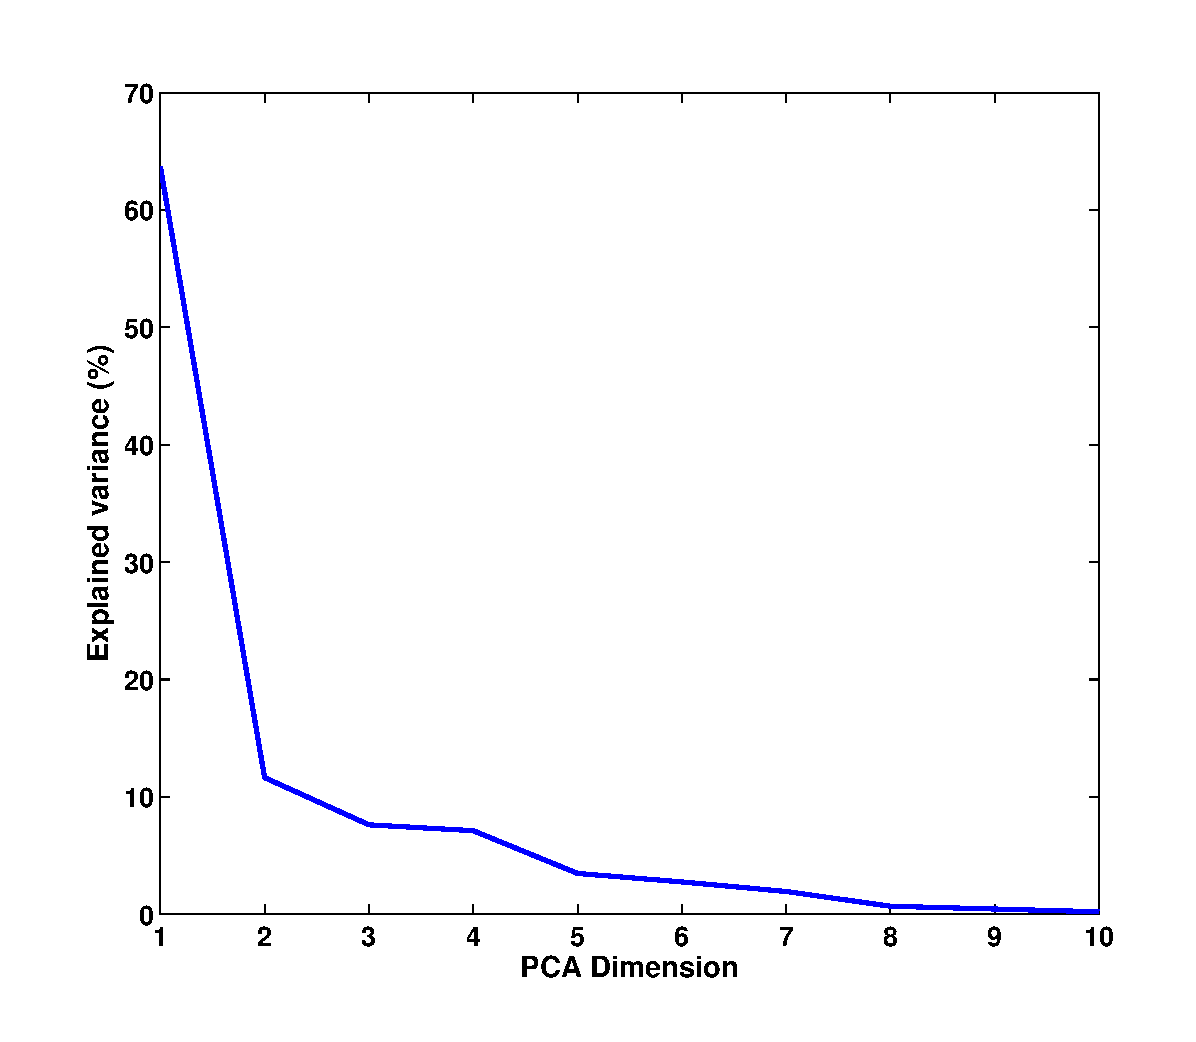
\includegraphics[width=62mm, height=52mm]{dia/gtvWholeEV.eps}}
    \caption{Isomap and PCA results for the 29 variable gearbox design
      problem pareto-front. Although the largest drop in residual variance
      is for two-dimensional embedding, it keeps dropping up to the fifth
      dimension. PCA explained variance shows four significant principal
      components.}
    \label{gtvRvEv}
  \end{center}
\end{figure}


Table \ref{first4GTVPCs} shows the variables with highest absolute weights
of first four principal components. There are no predominant variables in
the principal components, the weights are somewhat evenly distributed for
the first principal component. The second principal component, however, is 
dominated by the $p$ variable followed by gear teeth variables.


\begin{table}[!ht]
  \centering
  \begin{tabular}{|c|c|c|c|c|c|}
    \hline
    \multirow{2}{*}{First PC}   & $n_{16}$ &  $t_{5}$ &  $n_{8}$  & $n_{10}$ & $n_3$\\
    & 0.35  & 0.29  & 0.29 & 0.29 & 0.26  \\
    \hline
    \multirow{2}{*}{Second PC}   & $p$ &  $n_{2}$ &  $n_{16}$  & $n_{18}$ & $n_8$\\
    & -0.81 & -0.27 & -0.22 & -0.21 &  0.16 \\
    \hline
    \multirow{2}{*}{Third PC}   & $n_{11}$ &  $n_{9}$ &  $n_{5}$  & $n_{7}$ & $n_{3}$\\
    & -0.43 & -0.41 & 0.41 & -0.40 & 0.38 \\
    \hline
    \multirow{2}{*}{Fourth PC}   & $n_{12}$ &  $n_{10}$ &  $n_{8}$  & $n_{2}$ & $n_{4}$\\
    & 0.41 & 0.41 & 0.41 & -0.37 &  -0.33 \\
    \hline
  \end{tabular}
  \caption{Highest absolute weights of the first four principal components 
    of the gear train design problem (29 variables). There is no 
    dominant variable in the first principal component.}
  \label{first4GTVPCs}
\end{table}




\subsection{Analysis of the clusters}
 

\begin{figure}[ht]\begin{center}
 \subfloat[Clusters \textbf{A}, \textbf{C} and \textbf{E}.]{
 \label{gt11rv} 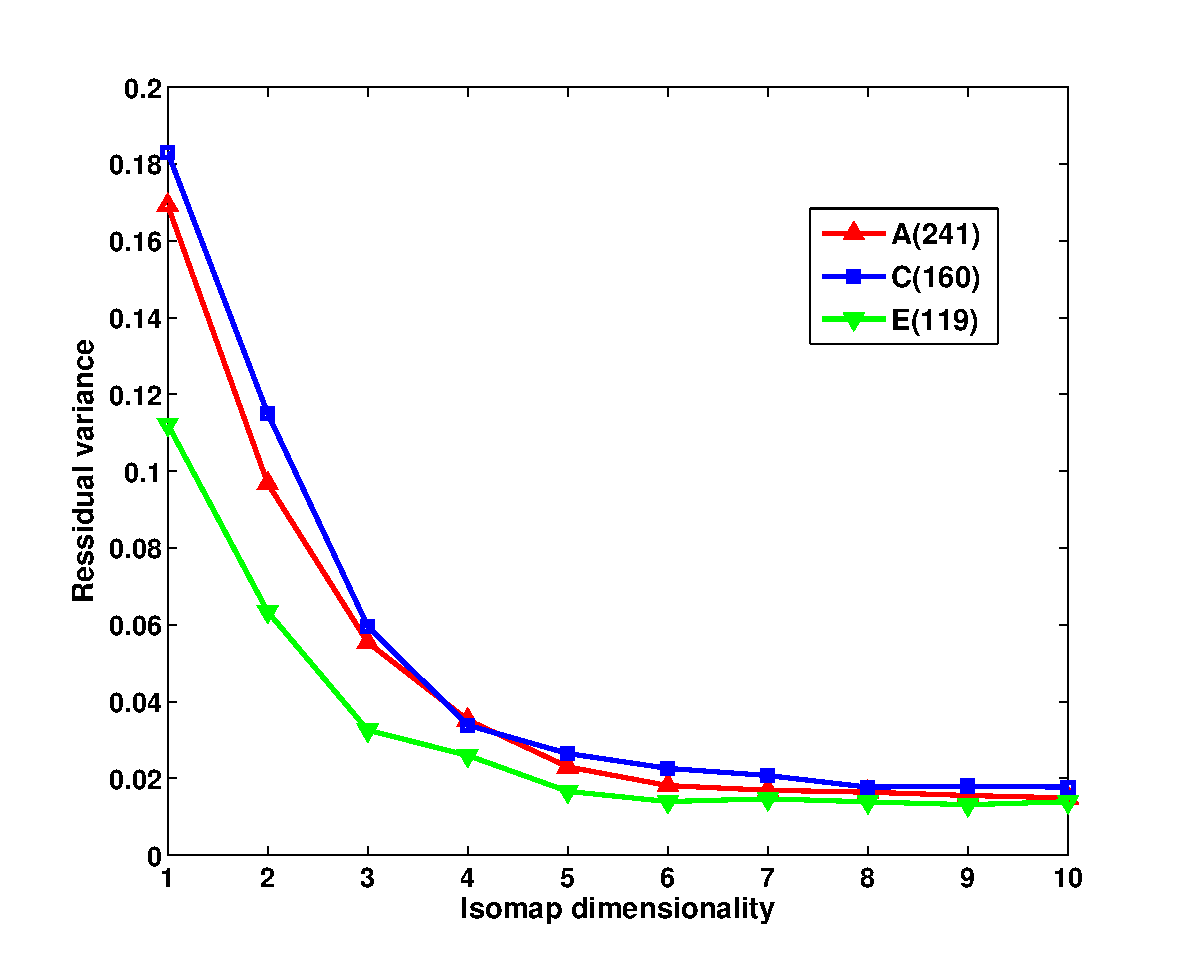
\includegraphics[width=62mm, height=52mm]{dia/gtvcrv1.eps}}
 \subfloat[Clusters \textbf{B}, \textbf{C}, \textbf{E} and \textbf{F}]{
 \label{gt11ev} 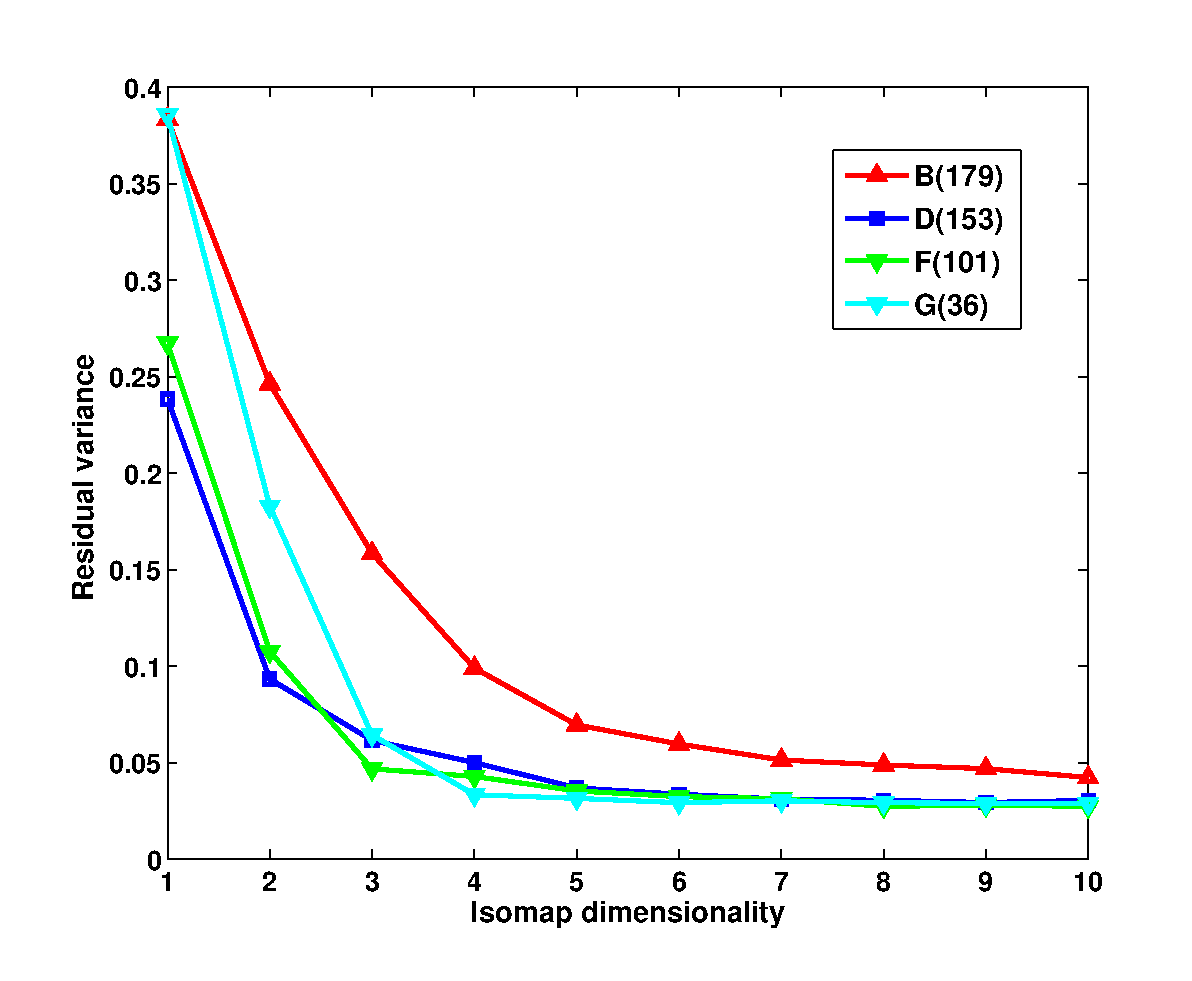
\includegraphics[width=62mm, height=52mm]{dia/gtvcrv2.eps}}
\caption{Isomap residual variances for clusters for the variable gear teeth
  problem. Residual variances for the clusters are similar to the whole
  pareto-front}
 \label{gtvClustersRV}
\end{center}\end{figure}

Cluster \textbf{A} has the largest number of optimal designs and occupies
the middle portion of the power range. Cluster \textbf{B} has the highest
power gearbox designs. \textbf{C} occupies the region between \textbf{A}
and \textbf{B}. All other clusters have low power gearbox designs with
\textbf{G} being the smallest and with the least power rating designs.
Having maximum output speed error as an objective doesn't provide any
additional useful choices to the designer, as this objective doesn't have
any trade-off or conflict with the other two objectives, turning this
optimization into essentially a two objective optimization.



The Isomap residual variances of the clusters shown in figure
\ref{gtvClustersRV} shows the clusters have manifold dimensionality similar
to the whole Pareto-front. The manifold dimensionality of the clusters
maybe 1 or 2 for most of the clusters though there are no precise
indications of the exact number of dimensions. The {\em minimization of
  error objective} in this case is an example of an {\em ill behaved}
objective function as discussed in section \ref{cdc} with reference to the
chunk dimensionality conjecture, as it doesn't monotonically increase or
decrease with the $n_{p_i}$ and $n_{w_i}$ variables. Nevertheless, the
dimensionality of the clusters are still in accordance with the conjectures
claim. The explained variance plots (figure \ref{gtvClustersEV}) present a
picture similar to that of the Isomap residual variances. The plots show
the cumulative explained variance of the principal components of the
clusters. For all the clusters the cumulative explained variance goes above
95\% only after the sixth principal component and the first three principal
components have quite significant explained variances.




\begin{figure}[ht]\begin{center}
 \subfloat[Clusters \textbf{A}, \textbf{B}, \textbf{C} and \textbf{D}]{
 \label{gt11rv} 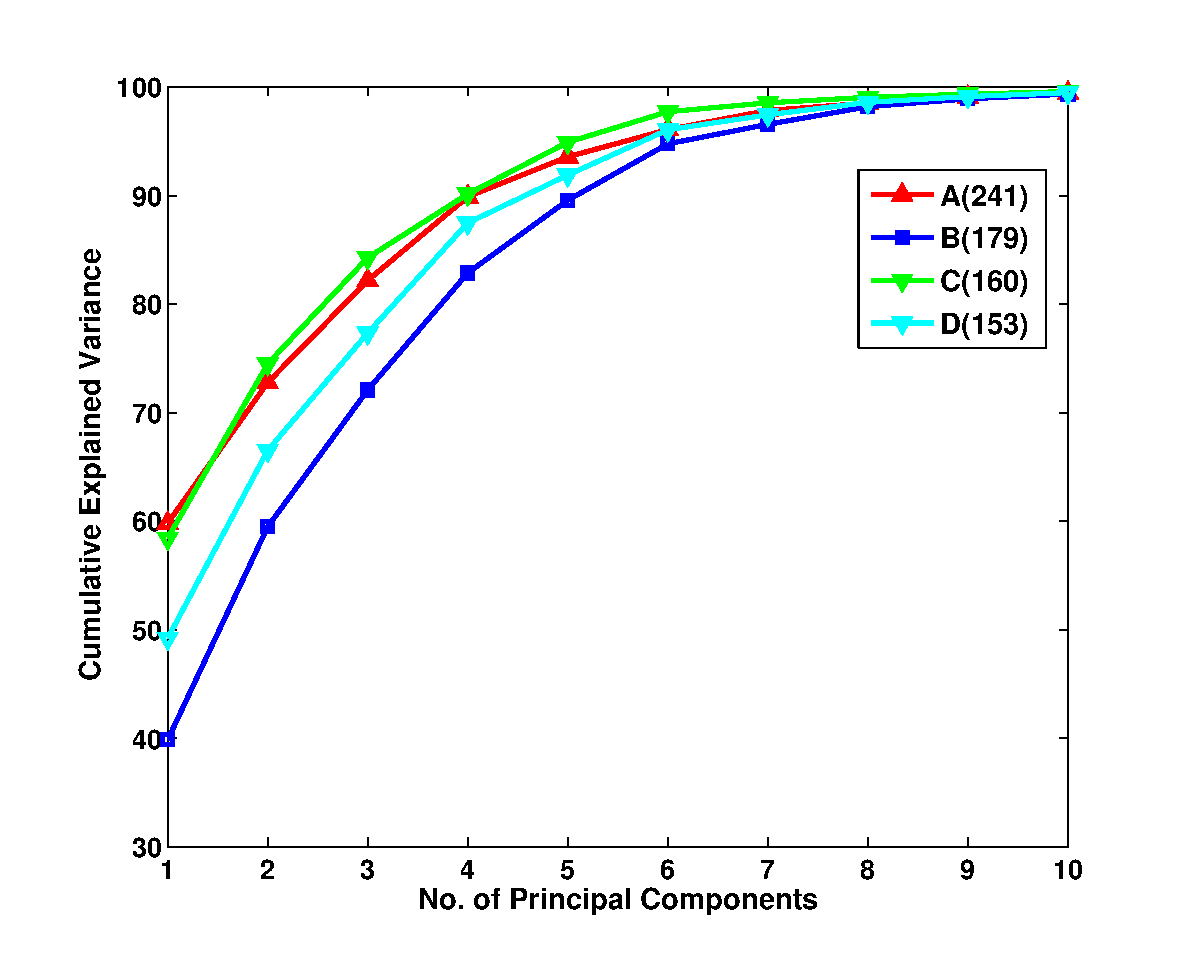
\includegraphics[width=62mm, height=52mm]{dia/gtvicev1.eps}}
 \subfloat[Clusters \textbf{E}, \textbf{F} and \textbf{G}]{
 \label{gt11ev} 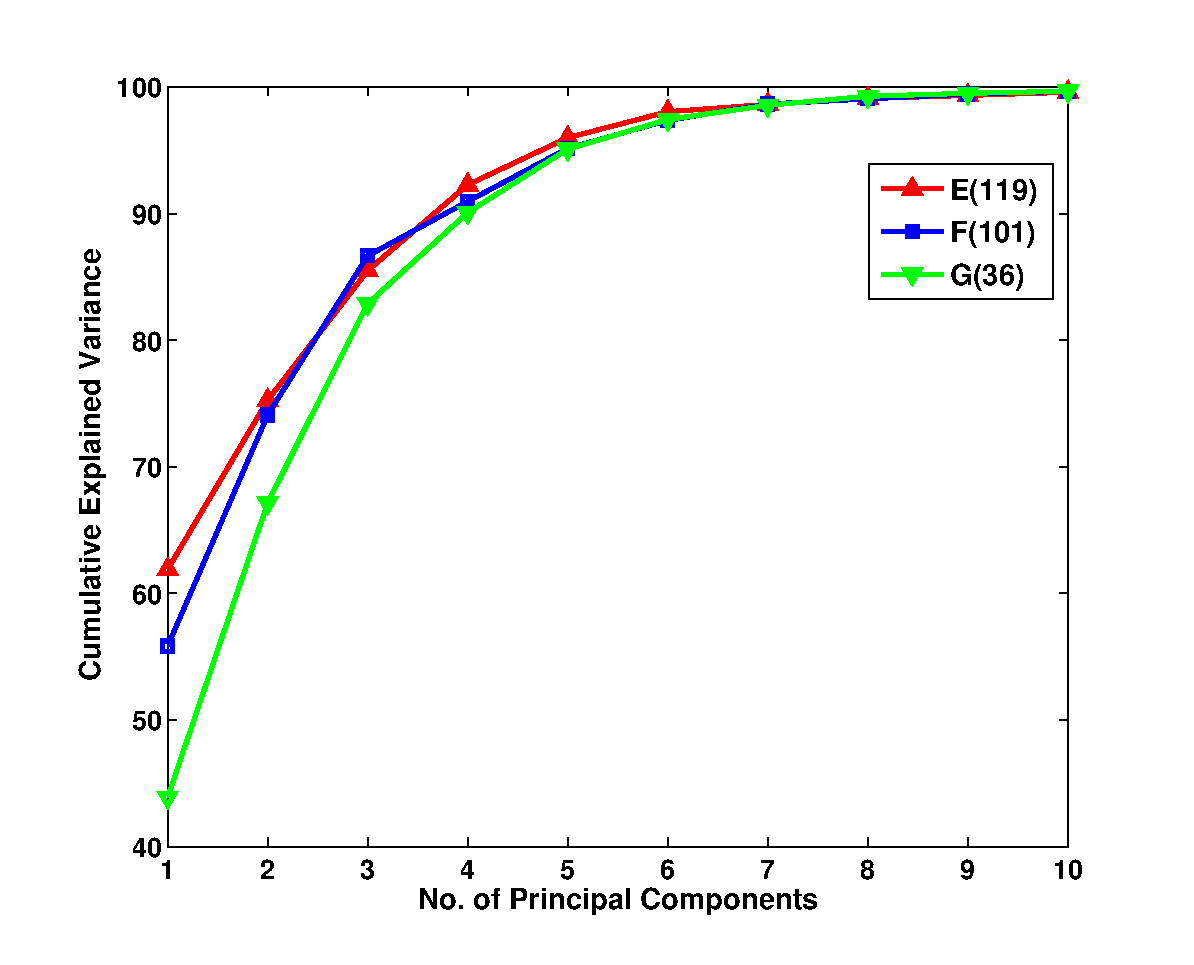
\includegraphics[width=62mm, height=52mm]{dia/gtvicev2.eps}}
 \caption{Cumulative PCA explained variance for 29 variable problem. For
  most clusters, first five-six principal components cover 90\% of the
  explained variance.}
 \label{gtvClustersEV}
\end{center}\end{figure}
 
In all the principal components number of teeth variables have the highest
weights. Unlike in the fixed layout gearbox design problem, power is not the 
dominant variable in the principal components. The $t_i$ variables have
weights lower than most of the number of the $n_i$ variables, except 
$n_{15}$, $n_{16}$, $n_{17}$ and $n_{18}$. Module is among the least important 
variables in all the principal components.

We have already explored the significance of the thickness variables and
module thickness in the pareto-front in the previous section. For this
reason, we will concentrate on the parts that the $n_i$ variables play in
the pareto-front clusters.  Table \ref{first2gtvnt} lists the $n_i$
variables in the sorted order of their absolute weights in the principal
components. The cells are shaded according to the transmission stage the
variable belongs to. The number of teeth variables of the second
transmission stage ($n_7$ to $n_{12}$) show the most amount of variability
while the last transmission stage has the most stable configuration showing
the least amount of variation in all the clusters.





   
{\tiny 

  \begin{table}[!ht]
    \centering
    \begin{tabular}{|c|c|c|c|c|c|c|c|c|c|c|c|c|}
      \hline
      \multirow{2}{*}{A} & First PC & \cellcolor[gray]{0.7} $n_{8}$ & \cellcolor[gray]{0.7} $n_{9}$ & \cellcolor[gray]{0.7} $n_{12}$ & \cellcolor[gray]{0.6} $n_{6}$ & \cellcolor[gray]{0.7} $n_{7}$ & \cellcolor[gray]{0.7} $n_{11}$ & $\dots$ & \cellcolor[gray]{0.9} $ n_{16}$ & \cellcolor[gray]{0.9} $n_{18}$ & \cellcolor[gray]{0.9} $n_{15}$ & \cellcolor[gray]{0.9} $n_{17}$ \\ \cline{2-13}
      & Second PC & \cellcolor[gray]{0.7} $n_{11}$ & \cellcolor[gray]{0.8} $n_{13}$ & \cellcolor[gray]{0.7} $n_{10}$ & \cellcolor[gray]{0.7} $n_{12}$ & \cellcolor[gray]{0.6} $n_{5}$ & \cellcolor[gray]{0.6} $n_{6}$ & $\dots$ & \cellcolor[gray]{0.9}  $n_{17}$ & \cellcolor[gray]{0.9}  $n_{16}$ & \cellcolor[gray]{0.9}  $n_{15}$ & \cellcolor[gray]{0.9} $n_{18}$ \\
      \hline
      \cline{1-13}
      \multirow{2}{*}{B}& First PC & \cellcolor[gray]{0.7} $n_{12}$ & \cellcolor[gray]{0.7} $n_{8}$ & \cellcolor[gray]{0.7} $n_{11}$ & \cellcolor[gray]{0.6} $n_{6}$ & \cellcolor[gray]{0.6} $n_{5}$ & \cellcolor[gray]{0.7} $n_{9}$ & $\dots$ & \cellcolor[gray]{0.9}  $n_{17}$ & \cellcolor[gray]{0.9}  $n_{15}$ & \cellcolor[gray]{0.9}  $n_{16}$ & \cellcolor[gray]{0.9} $n_{18}$ \\ 
      \cline{2-13}
      & Second PC & \cellcolor[gray]{0.7} $n_{11}$ & \cellcolor[gray]{0.7} $n_{10}$ & \cellcolor[gray]{0.7} $n_{8}$ & \cellcolor[gray]{0.7} $n_{12}$ & \cellcolor[gray]{0.6} $n_{6}$ & \cellcolor[gray]{0.8} $n_{13}$ & $\dots$ &  \cellcolor[gray]{0.9} $n_{15}$ & \cellcolor[gray]{0.9}  $n_{17}$ & \cellcolor[gray]{0.9} $n_{16}$ & \cellcolor[gray]{0.9} $n_{18}$ \\ 
      \hline
      \cline{1-13}
      \multirow{2}{*}{C}& First PC & \cellcolor[gray]{0.7} $n_{11}$ & \cellcolor[gray]{0.7} $n_{7}$ & \cellcolor[gray]{0.7} $n_{10}$ & \cellcolor[gray]{0.6} $n_{6}$ & \cellcolor[gray]{0.7} $n_{9}$ & \cellcolor[gray]{0.6} $n_{5}$ & $\dots$ &  \cellcolor[gray]{0.9}  $n_{17}$ & \cellcolor[gray]{0.9} $n_{18}$ & \cellcolor[gray]{0.9} $n_{15}$ & \cellcolor[gray]{0.9} $n_{16}$ \\ 
      \cline{2-13}
      & Second PC & \cellcolor[gray]{0.7} $n_{12}$ & \cellcolor[gray]{0.6} $n_{6}$ & \cellcolor[gray]{0.7} $n_{8}$ & \cellcolor[gray]{0.7} $n_{11}$ & \cellcolor[gray]{0.7} $n_{9}$ & \cellcolor[gray]{0.7} $n_{10}$ & $\dots$ &  \cellcolor[gray]{0.9}  $n_{15}$ & \cellcolor[gray]{0.9} $n_{16}$ & \cellcolor[gray]{0.9} $n_{18}$ & \cellcolor[gray]{0.9} $n_{17}$ \\ 
      \hline
      \cline{1-13}
      \multirow{2}{*}{D}& First PC & \cellcolor[gray]{0.7} $n_{9}$ & \cellcolor[gray]{0.7} $n_{8}$ & \cellcolor[gray]{0.7} $n_{10}$ & \cellcolor[gray]{0.6} $n_{5}$ & \cellcolor[gray]{0.7} $n_{12}$ & \cellcolor[gray]{0.7} $n_{7}$ & $\dots$ &  \cellcolor[gray]{0.9}  $n_{15}$ & \cellcolor[gray]{0.9} $n_{16}$ & \cellcolor[gray]{0.9} $n_{17}$ & \cellcolor[gray]{0.9}  $n_{18}$ \\ 
      \cline{2-13}
      & Second PC & \cellcolor[gray]{0.7} $n_{10}$ & \cellcolor[gray]{0.7} $n_{12}$ & \cellcolor[gray]{0.7} $n_{11}$ & \cellcolor[gray]{0.7} $n_{7}$ & \cellcolor[gray]{0.6} $n_{6}$ & \cellcolor[gray]{0.7} $n_{8}$ & $\dots$ &  \cellcolor[gray]{0.9} $n_{17}$ & \cellcolor[gray]{0.9} $n_{15}$ & \cellcolor[gray]{0.9} $n_{18}$ & \cellcolor[gray]{0.9}  $n_{16}$ \\ 
      \hline
      \cline{1-13}
      \multirow{2}{*}{E}& First PC & \cellcolor[gray]{0.7} $n_{8}$ & \cellcolor[gray]{0.7} $n_{9}$ & \cellcolor[gray]{0.7} $n_{12}$ & \cellcolor[gray]{0.6} $n_{6}$ & \cellcolor[gray]{0.7} $n_{11}$ & \cellcolor[gray]{0.8} $n_{13}$ & $\dots$ &  \cellcolor[gray]{0.9} $n_{18}$ & \cellcolor[gray]{0.9} $n_{17}$ & \cellcolor[gray]{0.9} $n_{15}$ & \cellcolor[gray]{0.9}  $n_{16}$ \\ 
      \cline{2-13}
      & Second PC & \cellcolor[gray]{0.7} $n_{9}$ & \cellcolor[gray]{0.7} $n_{8}$ & \cellcolor[gray]{0.7} $n_{12}$ & \cellcolor[gray]{0.7} $n_{7}$ & \cellcolor[gray]{0.7} $n_{10}$ & \cellcolor[gray]{0.6} $n_{4}$ & $\dots$ &  \cellcolor[gray]{0.9} $n_{16}$ & \cellcolor[gray]{0.9} $n_{15}$ & \cellcolor[gray]{0.9} $n_{17}$ & \cellcolor[gray]{0.9} $n_{18}$ \\ 
      \hline
      \cline{1-13}
      \multirow{2}{*}{F}& First PC & \cellcolor[gray]{0.7} $n_{11}$ & \cellcolor[gray]{0.7} $n_{9}$ & \cellcolor[gray]{0.6} $n_{6}$ & \cellcolor[gray]{0.7} $n_{8}$ & \cellcolor[gray]{0.6} $n_{5}$ & \cellcolor[gray]{0.7} $n_{7}$ & $\dots$ &  \cellcolor[gray]{0.9}  $n_{16}$ & \cellcolor[gray]{0.9}  $n_{15}$ & \cellcolor[gray]{0.9} $n_{18}$ & \cellcolor[gray]{0.9} $n_{17}$ \\ 
      \cline{2-13}
      & Second PC & \cellcolor[gray]{0.7} $n_{8}$ & \cellcolor[gray]{0.6} $n_{6}$ & \cellcolor[gray]{0.7} $n_{7}$ & \cellcolor[gray]{0.7} $n_{9}$ & \cellcolor[gray]{0.7} $n_{11}$ & \cellcolor[gray]{0.6} $n_{5}$ & $\dots$ &  \cellcolor[gray]{0.9} $n_{16}$ & \cellcolor[gray]{0.9} $n_{18}$ & \cellcolor[gray]{0.9} $n_{17}$ & \cellcolor[gray]{0.9} $n_{15}$ \\ 
      \hline
      \cline{1-13}
      \multirow{2}{*}{G}& First PC & \cellcolor[gray]{0.7} $n_{11}$ & \cellcolor[gray]{0.8} $n_{13}$ & \cellcolor[gray]{0.6} $n_{6}$ & \cellcolor[gray]{0.7} $n_{7}$ & \cellcolor[gray]{0.7} $n_{9}$ & \cellcolor[gray]{0.7} $n_{8}$ & $\dots$ &  \cellcolor[gray]{0.9} $n_{17}$ & \cellcolor[gray]{0.9} $n_{15}$ & \cellcolor[gray]{0.9} $n_{16}$ & \cellcolor[gray]{0.9}  $n_{18}$ \\ 
      \cline{2-13}
      & Second PC & \cellcolor[gray]{0.7} $n_{12}$ & \cellcolor[gray]{0.6} $n_{4}$ & \cellcolor[gray]{0.7} $n_{8}$ & \cellcolor[gray]{0.7} $n_{10}$ & \cellcolor[gray]{0.7} $n_{9}$ & \cellcolor[gray]{0.7} $n_{11}$ & $\dots$ &  \cellcolor[gray]{0.9}  $n_{17}$ & \cellcolor[gray]{0.9}  $n_{16}$ & \cellcolor[gray]{0.9} $n_{15}$ & \cellcolor[gray]{0.9} $n_{18}$ \\ 
      \hline
    \end{tabular}
    \caption{Ranking of gear teeth variables on the basis of absolute weights in principal components. The gear pairs of the last transmission stage occupy the last positions indicating they are the least varying.}
    \label{first2gtvnt}
  \end{table}
}


\subsection{Discussion}
Although power is still an objective in the multi-objective optimization,
 since there are three objectives (\emph{volume} and \emph{maximum error
  in output speeds} being the other two), a number of designs with same
power rating are possible, hence power is not a dominant variable in the
principal components. As observed earlier, having error as a third
objective isn't useful in the design process, as having higher error
apparently neither reduces the volume significantly nor improves the power
characteristics of the designs. 


\begin{figure}[ht]\begin{center}
 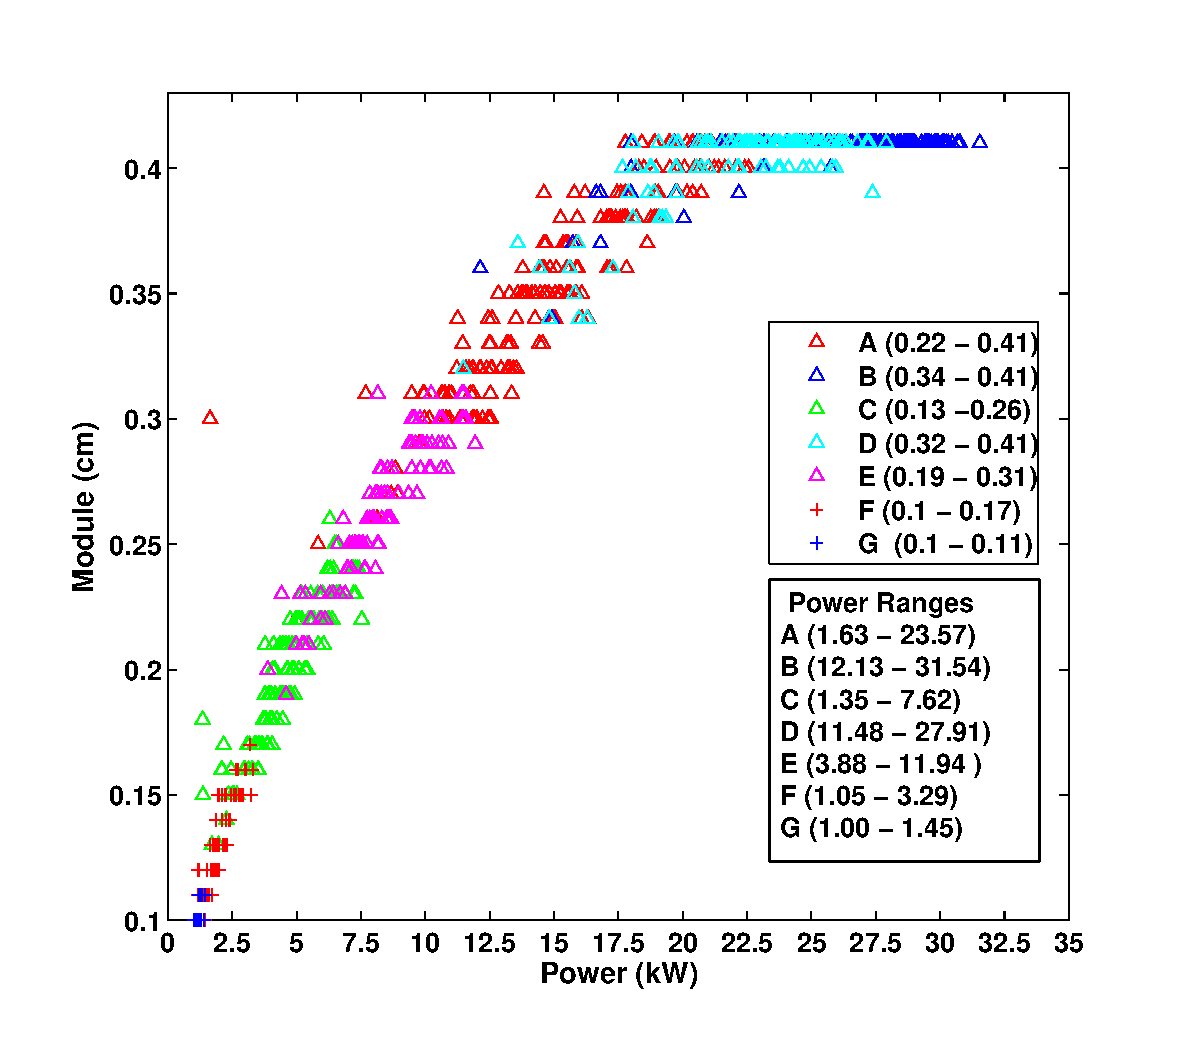
\includegraphics[width=100mm, height=80mm]{dia/gtvpVsm.eps}
 \caption{Power Vs. module characteristics of the pareto-front for 29
   variable problem. Clusters show intermingling unlike for the fixed layout
   problem.}
 \label{gtvpVsm}
\end{center}\end{figure}

The final transmission stage has to withstand the highest stresses, so the
module choice for the gear-box has to be able to withstand the stresses in
the final transmission stage. The same module is used in the gears of all
the transmission stages.  The number of teeth has to be kept minimum
possible as it also affects gearbox volume directly. Also there is a limit
on the maximum transmission ratio. All these trade-offs and limitations
lead to limited choices for the number of teeth variables in the final
transmission stage. On the other hand, in the second transmission stage
($n_{7}$ - $n_{12}$) has to withstand smaller stresses than the last stage,
it can meet the same stress requirements by increasing the number of teeth
and decreasing the gear pair thicknesses while maintaining the required
transmission ratios. This explains the positions of the number of teeth
variables in the last and second transmission stage.


The module to power characteristics are similar to the fixed layout case,
as shown in figure \ref{gtvpVsm}. Unlike in the previous case, designs
in different clusters can have the same module width. 


% \multirow{2}{*}{}& First PC & $n_{}$ & $n_{}$ & $n_{}$ & $n_{}$ & $n_{}$ & $n_{}$ & $\dots$ &  \cellcolor{} $n_{}$ & \cellcolor{} $n_{}$ & \cellcolor{}$n_{}$ & \cellcolor{} $n_{}$ \\ 
%\cline{2-13}
% & Second PC & $n_{}$ & $n_{}$ & $n_{}$ & $n_{}$ & $n_{}$ & $n_{}$ & $\dots$ &  \cellcolor{} $n_{}$ & \cellcolor{} $n_{}$ & \cellcolor{}$n_{}$ & \cellcolor{} $n_{}$ \\ 
%\hline
